\documentclass[]{elsarticle} %review=doublespace preprint=single 5p=2 column
%%% Begin My package additions %%%%%%%%%%%%%%%%%%%
\usepackage[hyphens]{url}



\usepackage{lineno} % add
\providecommand{\tightlist}{%
  \setlength{\itemsep}{0pt}\setlength{\parskip}{0pt}}

\usepackage{graphicx}
\usepackage{booktabs} % book-quality tables
%%%%%%%%%%%%%%%% end my additions to header

\usepackage[T1]{fontenc}
\usepackage{lmodern}
\usepackage{amssymb,amsmath}
\usepackage{ifxetex,ifluatex}
\usepackage{fixltx2e} % provides \textsubscript
% use upquote if available, for straight quotes in verbatim environments
\IfFileExists{upquote.sty}{\usepackage{upquote}}{}
\ifnum 0\ifxetex 1\fi\ifluatex 1\fi=0 % if pdftex
  \usepackage[utf8]{inputenc}
\else % if luatex or xelatex
  \usepackage{fontspec}
  \ifxetex
    \usepackage{xltxtra,xunicode}
  \fi
  \defaultfontfeatures{Mapping=tex-text,Scale=MatchLowercase}
  \newcommand{\euro}{€}
\fi
% use microtype if available
\IfFileExists{microtype.sty}{\usepackage{microtype}}{}
\bibliographystyle{elsarticle-harv}
\usepackage{longtable}
\ifxetex
  \usepackage[setpagesize=false, % page size defined by xetex
              unicode=false, % unicode breaks when used with xetex
              xetex]{hyperref}
\else
  \usepackage[unicode=true]{hyperref}
\fi
\hypersetup{breaklinks=true,
            bookmarks=true,
            pdfauthor={},
            pdftitle={Pervasive duplication of tumor suppressor genes preceded parallel evolution of large bodied Atlantogenatans},
            colorlinks=false,
            urlcolor=blue,
            linkcolor=magenta,
            pdfborder={0 0 0}}
\urlstyle{same}  % don't use monospace font for urls

\setcounter{secnumdepth}{5}
% Pandoc toggle for numbering sections (defaults to be off)


% Pandoc header
\usepackage{longtable}
\usepackage{booktabs}
\usepackage{geometry}
\usepackage{pdflscape}

\usepackage{float}
\let\origfigure\figure
\let\endorigfigure\endfigure
\renewenvironment{figure}[1][2] {
    \expandafter\origfigure\expandafter[H]
} {
    \endorigfigure
}
\usepackage{booktabs}
\usepackage{longtable}
\usepackage{array}
\usepackage{multirow}
\usepackage{wrapfig}
\usepackage{float}
\usepackage{colortbl}
\usepackage{pdflscape}
\usepackage{tabu}
\usepackage{threeparttable}
\usepackage{threeparttablex}
\usepackage[normalem]{ulem}
\usepackage{makecell}
\usepackage{xcolor}



\begin{document}
\begin{frontmatter}

  \title{Pervasive duplication of tumor suppressor genes preceded parallel evolution of large bodied Atlantogenatans}
    \author[University of Chicago]{Juan Manuel Vazquez}
  
    \author[SUNY Buffalo]{Vincent J Lynch}
  
      \address[University of Chicago]{Department of Human Genetics, 920 East 58th St, Chicago, IL, 60637}
    \address[SUNY Buffalo]{Department of Biological Sciences, 551 Cooke Hall, Buffalo NY, 14260}
    
  \begin{abstract}
  Cancer is an intrinsic disease of multicellular organisms. Within a species, the size of an animal, - correlated with the individual's number of cells - and its lifespan - correlated with increasing cellular damage over time - positively correlate with the risk any individual has to form tumors. Between species, however, we do not observe any correlation between size, lifespan, and cancer, a phenomenon that referred to as \emph{Peto's Paradox}. Elephants are a particularly interesting member of this class of paradoxical animals, since they are a set of large species deeply nested in a clade of smaller species, indicating a recent gain of size. Recent work has identified several individual cases of gene duplicates contributing to the increased cancer resistance of elephants, which suggests that duplication of tumor suppressor genes may play a more general role in mediating Peto's Paradox by increasing cancer resistance in large, long-lived species.
  By using a Reciprocal Best-Hit BLAT search approach, we investigated copy numbers of all protein-coding genes in \emph{Atlantogenatan} genomes to see if there is any correlation between the copy number of duplicates and changes body size along the phylogenetic tree. From an initial set of 18,011 protein-coding genes in hg38, we identified a median of 13,880 genes in \emph{Atlantogenatan} genomes, of which a median of 940 genes are duplicated. We find that, just as body size fluctuates throughout \emph{Atlantogenata}, genes involved in tumor suppressor pathways are also duplicated throughout the phylogenetic tree. Extant species of elephants, however, show active transcription of both canonical and duplicated copies of tummor suppressors that duplicated prior to and during their sudden increase in body size, suggesting that the duplication of tumor suppressor genes facilitates the evolution of increased body size by compensating for the increased cancer risk.
  \end{abstract}
  
 \end{frontmatter}

\hypertarget{introduction}{%
\section{Introduction}\label{introduction}}

Among the major constraints on the evolution of large body sizes (and long life-spans) in animals is an increased risk of developing cancer. If all cells in all organisms have a similar risk of malignant transformation and equivalent cancer suppression mechanisms, organism with many cells should have a higher prevalence of cancer than organisms with fewer cells, particularly because large and small animals have similar cell sizes ({[}1{]}). Consistent with this expectation there is a strong positive correlation between body size and cancer incidence within species, for example, cancer incidence increases with increasing adult height in humans {[}2,3{]} and in dogs {[}4,5{]}. There is no correlation, however, between body size and cancer risk \emph{between} species; this lack of correlation is often referred to as `Peto's Paradox' {[}6--8{]}. The ultimate resolution to Peto's Paradox is obvious: large bodied and long-lived species evolved enhanced cancer protection mechanisms. However, identifiying the specific genetic, molecular, and cellular mechanisms that underlie the evolution of augmented cancer protection has been difficult {[}9--13{]}.

Among the challenges for discovering how animals evolved enhanced cancer protection mechanisms is identifying lineages in which large bodied species are nested within species with small body sizes. \emph{Afrotherian} mammals are generally small-bodied, but also include the largest extant land mammals. For example, maximum adult weights are \textasciitilde{}70g in golden moles, \textasciitilde{}120g in tenrecs, \textasciitilde{}170g in elephant shrews, \textasciitilde{}3kg in hyraxes, and 60kg in aardvarks {[}14{]}. While extant hyraxes are relatively small, the extinct Titanohyrax is estimated to have weighted up to \textasciitilde{}1300kg {[}15{]}. The largest members of \emph{Afrotheria}, too, are dwarfed by the size of their recent ancestors: extant cows manatees are large bodied (\textasciitilde{}322-480kg) but are relatively small compared to the extinct Stellar's sea cow which is estimated to have weight 8000-10000kg {[}16{]}. Similarly African (4,800kg) and Asian elephants (3,200kg) are the largest living elephant species, but are dwarfed by the truly gigantic extinct Proboscideans such as Deinotherium (\textasciitilde{}132,000kg), Mammut borsoni (110,000kg), and the Asian straight-tusked elephant (\textasciitilde{}220,000kg), the largest known land mammal {[}17{]}. Remarkably, these large-bodied \emph{Afrotherian} lineages are nested within small bodied species (\textbf{Figure \ref{fig:Figure-intro}}) {[}18--21{]}, indicating that gigantism independently evolved in hyraxes, sea cows, and elephants (\emph{Paenungulata}). Thus, Paenungulates are an excellent model system in which to explore the mechanisms that underlie the evolution of large body sizes and augmented cancer resistance.

Although many mechanisms can potentially resolve Peto's paradox, among the most parsimonious routes to enhanced cancer resistance is through an increased copy number of tumor suppressors. Indeed, candidate genes studies have found that the elephant genome encodes duplicate such as \emph{TP53} and \emph{LIF} {[}13,22,23{]} as well as other genes with putative tumor suppressive functions {[}24,25{]}. As these studies focus on \emph{a priori} gene sets, however, it remains unknown whether this is a general, genome-wide trend in \emph{Afrotherian} genomes; and whether such a general trend is associated with the recent increases in body size -- and therefore expected cancer risk -- in these species.

Here, we trace the evolution of body mass and gene copy number variation in across \emph{Afrotherian} genomes in order to investigate whether duplication of tumors suppresor is common in large, long-lived Proboscideans. Our estimates of the evolution of body mass, similarly to previous studies {[}18--21{]}, show that large body masses evolved in a step-wise manner, with major increases in body mass in the \emph{Pseudoungulata} (17kg), \emph{Paenungulata} (25kg), \emph{Tethytheria} (296kg), and \emph{Proboscidea} (4,100kg) stem-lineages. To explore whether duplication of tumor suppressor genes occurred coincident with the evolution of large body sizes, we used a genome-wide Reciprocal Best BLAT Hit (RBBH) strategy to identify gene duplications, and used maximum likelihood to infer the lineages in which those duplications occurred. Unexpectedly, we found that duplication of tumor suppressor genes was common in all Afrotherians, both large and small. These data suggest that duplication of tumor suppressor genes is pervasive in Afrotherians and proceeded the evolution of species with very large body sizes.

\hypertarget{methods}{%
\section{Methods}\label{methods}}

\hypertarget{ancestral-body-size-reconstruction}{%
\subsection{Ancestral Body Size Reconstruction}\label{ancestral-body-size-reconstruction}}

We built a time-calibrated supertree of Eutherian mammals by combining the time-calibrated molecular phylogeny of Bininda-Emonds \emph{et al.} {[}26{]} with the time-calibrated total evidence Afrotherian phylogeny from Puttick and Thomas {[}21{]}. While the Bininda-Emonds \emph{et al.} {[}26{]} phylogeny includes 1,679 species, only 34 are Afrotherian, and no fossil data are included. The inclusion of fossil data from extinct species is essential to ensure that ancestral state reconstructions of body mass are not biased by only including extant species. This can lead to inaccurate reconstructions, for example, if lineages convergently evolved large body masses from a small bodied ancestor. In contrast, the total evidence Afrotherian phylogeny of Puttick and Thomas {[}21{]} includes 77 extant species and fossil data from 39 extinct species. Therefore we replaced the Afrotherian clade in the Bininda-Emonds \emph{et al.} {[}26{]} phylogeny with the Afrotherian phylogeny of Puttick and Thomas {[}21{]} using Mesquite. Next, we jointly estimated rates of body mass evolution and reconstructed ancestral states using a generalization of the Brownian motion model that relaxes assumptions of neutrality and gradualism by considering increments to evolving characters to be drawn from a heavy-tailed stable distribution (the ``Stable Model'') implemented in StableTraits {[}27{]}. The stable model allows for occasional large jumps in traits and has previously been shown to out-perform other models of body mass evolution, including standard Brownian motion models, Ornstein--Uhlenbeck models, early burst maximum likelihood models, and heterogeneous multi-rate models {[}27{]}.

\hypertarget{identification-of-duplicate-genes}{%
\subsection{Identification of Duplicate Genes}\label{identification-of-duplicate-genes}}

\textbf{Reciprocal Best-Hit BLAT:} We developed a reciprocal best hit BLAT (RBHB) pipeline to identify putative homologs and estimate gene copy number across species (\ref{fig:Figure-RBHBStrategy}). The Reciprocal Best Hit (RBH) search strategy is conceptually straightforward: 1) Given a gene of interest \(G_A\) in a query genome \(A\), one searches a target genome \(B\) for all possible matches to \(G_A\); 2) For each of these hits, one then performs the reciprocal search in the original query genome to identify the highest-scoring hit; 3) A hit in genome \(B\) is defined as a homolog of gene \(G_A\) if and only if the original gene \(G_A\) is the top reciprocal search hit in genome \(A\). We selected BLAT {[}28{]} as our algorithm of choice, as this algorithm is sensitive to highly simliar (\textgreater{}90\% identity) sequences, thus identifying the highest-confidence homologs while minimizing many-to-one mapping problems when searching for multiple genes. RBH performs similar to other more complex methods of orthology prediction, and is particularly good at identifying incomplete genes that may be fragmented in low quality/poor assembled regions of the genome {[}29,30{]}.

\textbf{Effective Copy Number By Coverage:} In lower-quality genomes, many genes are fragmented across multiple scaffolds, which results in BLAT calling multiple hits when in reality there is only one gene. To compensate for this, we came up with a novel statistic, Estimated Copy Number by Coverage (ECNC), which averages the number of times we see each nucleotides of a query sequence in a target genome over the total number of nucleotides of the query sequence found overall in each target genome (\textbf{Figure \ref{fig:Figure-ECNC}}). This allows us to correct for genes that have been fragmented across incomplete genomes, while also taking into account missing sequences from the human query in the target genome. Mathematically, this can be written as:\\
\[ ECNC = \frac{\sum_{n=1}^{l} C_n}{\sum_{n=1}^{l} bool(C_n)}\]
where \(n\) is a given nucleotide in the query, \(l\) is the total length of the query, \(C_n\) is the number of instances that \(n\) is present within a reciprocal best hit, and \(bool(C_n)\) is 1 if \(C_n > 0\) or 0 if \(C_n = 0\).

\textbf{RecSearch Pipeline:} We created a custom Python pipeline for automating RBHB searches between a single reference genome and multiple target genomes using a list of query sequences from the reference genome. For the query sequences in our search, we used the hg38 Proteome provided by UniProt {[}31{]}, which is a comprehensive set of protein sequences curated from a combination of predicted and validated protein sequences generated by the UniProt Consortium. In order to refine our search, we omitted protein sequences originating from long, noncoding RNA loci (e.g.~LINC genes); poorly-studied genes from predicted open reading frames (C-ORFs); and sequences with highly repetitive sequences such as zinc fingers, protocadherins, and transposon-containing genes, as these were prone to high levels of false positive hits.

After filtering out problematic protein queries (see below), we then used our pipeline to search for all copies of our 18011 query genes in publicly available \emph{Afrotherian} genomes (\ref{tab:Table-Genomes}), including African savannah elephant (\emph{Loxodonta africana}: loxAfr3, loxAfr4, loxAfrC), African forest elephant (\emph{Loxodonta cyclotis}: loxCycF), Asian Elephant (\emph{Elephas maximus}: eleMaxD), Woolly Mammoth (\emph{Mammuthus primigenius}: mamPriV), Colombian mammoth (\emph{Mammuthus columbi}: mamColU), American mastodon (\emph{Mammut americanum}: mamAmeI), Rock Hyrax (\emph{Procavia capensis}: proCap1, proCap2, proCap2\_HiC), West Indian Manatee (\emph{Trichechus manatus latirostris}: triManLat1, triManLat1\_HiC), Aardvark (\emph{Orycteropus afer}: oryAfe1, oryAfe1\_HiC), Lesser Hedgehog Tenrec (\emph{Echinops telfairi}: echTel2), Nine-banded armadillo (\emph{Dasypus novemcinctus}: dasNov3), Hoffman's two-toed sloth (\emph{Choloepus hoffmannii}: choHof1, choHof2, choHof2\_HiC), Cape golden mole (\emph{Chrysochloris asiatica}: chrAsi1), and Cape elephant shrew (\emph{Elephantulus edwardii}: eleEdw1).

\textbf{Query gene inclusion criteria:} To assemble our query list, we first removed all unnamed genes from UP000005640. Next, we excluded genes from downstream analyses for which assignment of homology was uncertain, including uncharacterized ORFs (991 genes), LOC (63 genes), HLA genes (402 genes), replication dependent histones (72 genes), odorant receptors (499 genes), ribosomal proteins (410 genes), zinc finger transcription factors (1983 genes), viral and repetitive-element-associated proteins (82 genes) and any protein described as either ``Uncharacterized,'' ``Putative,'' or ``Fragment'' by UniProt in UP000005640 (30724 genes), leaving us with a final set of 37582 query protein isoforms, corresponding to 18011 genes.

\textbf{Duplication gene inclusion criteria:} In order to condense transcript-level hits into single gene loci, and to resolve many-to-one genome mappings, we removed exons where transcripts from different genes overlapped, and merged overlapping transcripts of the same gene into a single gene locus call. The resulting gene-level copy number table was then combined with the maximum ECNC values observed for each gene in order to call gene duplications. We called a gene duplicated if its copy number was two or more, and if the maximum ECNC value of all the gene transcripts searched was 1.5 or greater; previous studies have shown that incomplete duplications can encode functional genes {[}13,23{]}, therefore partial gene duplications were included provided they passed additional inclusion criteria (see below). The ECNC cut off of 1.5 was selected empirically, as this value minimized the number of false positives seen in a test set of genes and genomes. The results of our initial search are summarized in Figure \ref{fig:Figure-GeneDup-Cladogram}. Overall, we identified 13880 genes across all species, or 77.1\% of our starting query genes.

\textbf{Genome Quality Assessment using CEGMA:} In order to determine the effect of genome quality on our results, we used the gVolante webserver and CEGMA to assess the quality and completeness of the genome {[}32,33{]}. CEGMA was run using the default settings for mammals (``Cut-off length for sequence statistics and composition'' = 1;``CEGMA max intron length'' = 100000; ``CEGMA gene flanks'' = 10000, ``Selected reference gene set'' = CVG). For each genome, we generated a correlation matrix using the aforementioned genome quality scores, and either the mean Copy Number or mean ECNC for all hits in the genome.

\hypertarget{evidence-for-functionality-of-gene-duplicates}{%
\subsection{Evidence for Functionality of Gene Duplicates}\label{evidence-for-functionality-of-gene-duplicates}}

To validate and filter out duplicate gene calls, we intersected our results with either gene prediction or transcriptomic evidence as a proxy for functionality.

\textbf{Transcriptome Assembly:} For the African Savana Elephant, Asian Elephant, West Indian Manatee, and Nine-Banded Armadillo, we generated \emph{de novo} transcriptomes using publically-available RNA-sequencing data from NCBI SRA (\ref{tab:Table-SRAData}). We mapped reads to all genomes available for each species, and assembled transcripts using HISAT2 and StringTie, respectively {[}34--36{]}. RNA-sequencing data was not available for Cape Golden Mole, Cape Elephant Shrew, Rock Hyrax, Aardvark, or the Lesser Hedgehog Tenrec.

\textbf{Gene Prediction:} We obtained tracks for genes predicted using GenScan for all the genomes available via UCSC Genome Browser: African savannah elephant (loxAfr3), Rock Hyrax (proCap1), West Indian Manatee (triManLat1), Aardvark (oryAfe1), Lesser Hedgehog Tenrec (echTel2), Nine-banded armadillo (dasNov3), Hoffman's Two-Toed Sloth (choHof1), Cape golden mole (chrAsi1), and Cape Elephant Shrew (eleEdw1); gene prediction tracks for higher-quality assemblies were not available.

\textbf{Evidenced Duplicate Criteria:} We intersected our records of duplicate hits identified in each genome with the gene prediction tracks and/or transcriptome assemblies using \texttt{bedtools}. When multiple lines of evidence for functionality were present for a genome, we used the union of all intersections as the final output for evidenced duplicates. When analyzing the highest-quality assemblies available for each species, if a species had neither gene prediction tracks nor RNA-seq data for the highest-quality genome available, we conservatively included all hits for the genome in the final set of evidenced duplicates.

\hypertarget{reconstruction-of-ancestral-copy-numbers}{%
\subsection{Reconstruction of Ancestral Copy Numbers}\label{reconstruction-of-ancestral-copy-numbers}}

We encoded the copy number of each gene for each species as a discrete trait ranging from 0 (one gene copy) to 31 (for 32+ gene copies) and used IQ-TREE to select the best-fitting model of character evolution {[}37--41{]}, which was inferred to be a Jukes-Cantor type model for morphological data (MK) with equal character state frequencies (FQ) and rate heterogeneity across sites approximated by including a class of invariable sites (I) plus a discrete Gamma model with four rate categories (G4). Next we inferred gene duplication and loss events with the empirical Bayesian ancestral state reconstruction (ASR) method implemented in IQ-TREE {[}37--41{]}, the best fitting model of character evolution (MK+FQ+GR+I) {[}42,43{]}, and the unrooted species tree for Atlantogenata. We considered ancestral state reconstructions to be reliable if they had Bayeisan Posterior Probability (BPP) ?0.80; less reliable reconstructions were excluded for pathway analyses.

\hypertarget{pathway-enrichment-analysis}{%
\subsection{Pathway Enrichment Analysis}\label{pathway-enrichment-analysis}}

To determine if gene duplications were enriched in particular biological pathways, we used the WEB-based Gene SeT AnaLysis Toolkit (WEBGESTALT){[}44{]} to perform overrepresentation analysis (ORA); pathway databases included Reactome {[}45{]}, Wikipathways, {[}46{]}, and KEGG {[}47{]}. Gene duplicates in each lineage were used as the foreground gene set, and the initial query set was used as the background gene set. Statistical significance of enriched terms was assessed with a hypergeometric test, and controlled for multiple testing using the Benjamini-Hochberg false discovery rate (FDR); each analysis was run at FDR=0.1, FDR=0.2, FDR=0.3, and FDR=0.5. In order to determine an empirical false positive rate for term enrichment, we randomly sampled 1000-10,000 genes from our background set 1000 times, and ran the aforementioned analyses to see which terms were likely to randomly appear; there were no terms which appeared at FDR \(\leq\) 0.3.

\hypertarget{estimating-the-evolution-of-cancer-risk}{%
\subsection{Estimating the Evolution of Cancer Risk}\label{estimating-the-evolution-of-cancer-risk}}

The dramatic increase in body mass and lifespan in some Afrotherian lineages implies those lineages must have also evolved reduced cancer risk. To infer the magnitude of these reductions we estimated differences in intrinsic cancer risk across extant and ancestral Afrotherians. Following Peto {[}48{]} we estimate the intrinsic cancer risk as the product of risk associated with body mass and lifespan. In order to determine the intrinsic cancer risk (\(K\)) across species and at ancestral nodes (see below), we first needed to estimate ancestral lifespans at each node. We used Phylogenetic Generalized Least-Square Regression (PGLS) {[}49,50{]} implemented in the R package \texttt{ape} to calculate estimated ancestral lifespans across \emph{Atlantogenata} using our estimates for body size at each node. In order to estimate the intrinsic cancer risk of a species, we first inferred lifespans at ancestral nodes using PGLS and the model \(ln(lifespan) = \beta_{1}corBrowninan + \beta_{2}ln(size) + \epsilon\). Next, we calculated \(K_{1}\) at all nodes, and then estimated the fold change in cancer susceptibility between ancestral and descendant nodes (Figure \ref{fig:Figure-CancerSuscept}, Table \ref{tab:Table-CancerSuscept}).A Next, in oder to calculate \(K_{1}\) at all nodes, we used a simplified multistage cancer risk model for body size \(D\) and lifespan \(t\): \(K \approx Dt^6\) {[}8,48,51,52{]}. The fold change in cancer risk between a node and its ancestor was then defined as \(\log_{2}(\frac{K_{2}}{K_{1}})\).

\hypertarget{results}{%
\section{Results}\label{results}}

\hypertarget{step-wise-evolution-of-body-size-in-afrotherians}{%
\subsection{\texorpdfstring{Step-wise evolution of body size in \emph{Afrotherians}}{Step-wise evolution of body size in Afrotherians}}\label{step-wise-evolution-of-body-size-in-afrotherians}}

Similar to previous studies of Afrotherian body size {[}21,27{]}, we found that the body mass of the Afrotherian ancestor was inferred to be small (0.26kg, 95\% CI: 0.31-3.01kg) and that substantial accelerations in the rate of body mass evolution occurred coincident with a 67.36x increase in body mass in the stem-lineage of \emph{Pseudoungulata} (17.33kg), a 1.45x increase in body mass in the stem-lineage of \emph{Paenungulata} (25.08kg), a 11.82x increase in body mass in the stem-lineage of \emph{Tehthytheria} (296.56kg), and a 2.69x increase in body mass in the stem-lineage of \emph{Proboscidea} (4114.39kg) (Figure \ref{fig:Figure-BodySize}, Table \ref{tab:Table-BodySize}). The ancestral \emph{Hyracoidea} was inferred to be relatively small (2.86kg-118.18kg), and rate accelerations were coincident with independent body mass increases in large hyraxes such as \emph{Titanohyrax andrewsi} (429.34kg, 67.36x increase). While the body mass of the ancestral \emph{Sirenian} was inferred to be large (61.7kg-955.51kg), a rate acceleration occurred coincident with a 10.59x increase in body mass in Stellar's sea cow. Rate accelerations also occurred coincident with 36.6x decrease in body mass in the stem-lineage of the dwarf elephants \emph{Elephas (Palaeoloxodon) antiquus falconeri} and \emph{Elephas cypriotes}. These data suggest that gigantism in \emph{Afrotherians} evolved step-wise, from small to medium bodies in the \emph{Pseudoungulata} stem-lineage, medium to large bodies in the \emph{Tehthytherian} stem-lineage and extinct hyraxes, and from large to exceptionally large bodies independently in the \emph{Proboscidean} stem-lineage and Stellar's sea cow (Figure \ref{fig:Figure-BodySize}, Table \ref{tab:Table-BodySize}).

\hypertarget{step-wise-reduction-of-intrinsic-cancer-risk-in-large-long-lived-afrotherians}{%
\subsection{Step-wise reduction of intrinsic cancer risk in large, long-lived Afrotherians}\label{step-wise-reduction-of-intrinsic-cancer-risk-in-large-long-lived-afrotherians}}

As expected, intrinsic cancer susceptibility in Afrotheria also varies with changes in body size and longevity (Figure \ref{fig:Figure-CancerSuscept}, Table \ref{tab:Table-CancerSuscept}), with an initial 9.22-fold and 20.75-fold increase in the stem-lineage of Afrotheria and Xenarthra, respectively, followed by a 9.22-fold increases in Pseudoungulata and a 5.38-fold increase in Aardvarks (Figure \ref{fig:Figure-CancerSuscept}, Table \ref{tab:Table-CancerSuscept}). In contrast to the Paenungulate stem-lineage, there is a 6.92-fold increase in cancer risk in Tethytheria, a 8.62-fold increase in Manatee, and dramatic increases within Proboscidea including a 27.66-fold increase in Elephantidae and a 29.97-fold in the American Mastodon. Within the Elephantidae, Elephantina and Loxodontini have a 2.31-fold increase in cancer susceptibility, while susceptibility is relatively stable in Mammoths. The three extant Proboscideans, Asian Elephant, African Savana Elephant, and the African Forest Elephant, meanwhile, have similar decreases in both size and cancer susceptibility (Figure \ref{fig:Figure-CancerSuscept}, Table \ref{tab:Table-CancerSuscept}).

\hypertarget{identification-and-evolutionary-history-of-gene-duplications}{%
\subsection{Identification and evolutionary history of gene duplications}\label{identification-and-evolutionary-history-of-gene-duplications}}

We found that gene duplications were common in Atlantogenatan genomes (Figure \ref{fig:Figure-GeneDup-Cladogram}), identifying an average of NA genes, with an average of 10.53\% duplicated; this is in-line with other studies describing the rates of gene duplications over time. {[}53{]}. We observed that the percentage of duplicated genes in non-\emph{Pseudoungulatan} genomes was significantly higher: while \emph{Pseudoungulatan} genomes had duplicates percentages ranging anywhere from 3.26\% to 7.80\%, outgroup species' duplication rates ranged from 12.94\% to 23.66\%. To explore whether genome quality may adversely effect our inferences, we used CEGMA and the gVolante server {[}32,33{]} to assess the correlation between genome quality and copy number estimates. As shown in Figure \ref{fig:Figure-GenomeCor}, mean Copy Number, mean ECNC, and mean CN (the lesser of Copy Number and ECNC per gene) moderately or strongly correlate with genomic quality, such as LD50, the number of scaffolds, and contigs with a length above either 100K or 1M.

Among the genes that increased in copy number in the elephant lineage are TP53 and LIF, as previously described; however, we find that these two genes represent a fraction of the 940 genes that are duplicated in the African Elephant overall, which accumulated over various steps through their evolution. While the extinct elephantids have acceptable genome quality metrics according to CEGMA, they are nonetheless missing a significant number of sequences; this may contribute to the low number of duplicated genes that occured in internal nodes. The number of duplicates that occur at each branch is also proportional to the density of the sampling of the clade overall, as would be expected. In branches, such as \emph{Afrosoricida}, where the number of species is relatively minuscule compared to the size of the clade, we see many significantly larger numbers of duplications private to these species.

\hypertarget{duplications-that-occurred-recently-in-probodiscea-are-enriched-for-tumor-suppressor-pathways}{%
\subsection{Duplications that occurred recently in Probodiscea are enriched for tumor suppressor pathways}\label{duplications-that-occurred-recently-in-probodiscea-are-enriched-for-tumor-suppressor-pathways}}

Our initial hypothesis was that genes which duplicated in lineages that experienced a growth in size would be enriched for membership in tumor suppressor pathways. Thus, we used WebGestalt and its Overrepresentation Analysis (ORA) functionality to determine what pathways were enriched in our duplicated gene sets in each branch relative to our initial query set. For our database, we used Reactome for our primary analysis, but additionally used the KEGG, Panther, Wikipathways, and Wikipathways\_cancer databases using WebGestalt ORA. Going through the tree, at no FDR \(\leq\) 0.5 is there any significant pathway representation for genes that increased in the branches leading to \emph{Afrosoricida}, \emph{Pseudoungulata}, \emph{Elephantina}, \emph{Loxodontini}, \emph{Elephas maximus}, \emph{Mammuthus}, \emph{Loxodonta cyclotis}, \emph{Palaeoloxodon antiquus}, \emph{Loxodona}, \emph{Mammuthus columbi}, \emph{Mammuthus primigenius}, \emph{Procavia capensis}, \emph{Elephantidae}, or \emph{Proboscidea}; furthermore, there are no significant pathway enrichments at FDR\textless{}0.5 for genes whose copy number did not change between branches (copy-number-stable) for \emph{Afrotheria}. Note that because \emph{Xenarthra} was selected as the outgroup, it is not possible to polarize the changes in their gene copy numbers along the tree.

For the other branches, the number of pathways that came up as significantly enriched at each FDR is shown in Table \ref{tab:Table-OraFreqDatabase}. For the species with high duplication rates and lower-quality, highly-fragmented genomes, such as with \emph{Chrysochloris asiatica} (20.05\% duplicated hits) and \emph{Elephantulus edwardii} (23.66\% duplicated hits), it is unsurprising that there is a proportionally large number of pathway enrichments. In the case of these two species, their many pathway enrichments also span an incredible range of processes at every level of biology; this, in combination with the high number of copy numbers identified for these genes, further suggests a need for improvement and refinement in these genomes. In the cell cycle pathways called as significant in the genomes of these two species plus \emph{Orycteropus afer} and \emph{Echinops telfairi}, the duplicated genes included in these sets are from the same gene families, such as the APC subunit family; the proteosome subunit families; and the protein phosphatase 2 family, among others. It is highly possible that these results reflect true expansions of these gene families, especially in the higher-quality \emph{Orycteropus afer} genome; however, it is also possible that it simply reflects artifactual duplications, and so require further study.

The pathway enrichments for genes whose copy number either did not change, or whose copy number increased, between \emph{Loxodona} and the African Elephant are shown in Figure \ref{fig:Figure-loxAfrORA}. Among the few enriched pathways in the African Elephant, we see that that two tumor suppression pathways - APC Complex-related pathways, and ``TP53 Regulates Metabolic Genes''- appear not only in the case of stable genes, but also in the set of newly duplicated genes. The other pathways we see in the set of recently-duplicated genes include ``Functionalization of Compounds'' and its daughter pathway ``Xenobiotics''. Genes in these pathways serve to add functional groups to lipophylic compounds which would otherwise not be reactive in the cell, and are types of metabolic pathways. In the stable set we see enrichment of pathways such as ``Neuronal Systems'' and ``Axon Guidance,'' which fit in well with what is known about elephant biology and evolution {[}54{]}. Overall in elephants, we see enrichments within duplicated genes for pathways involved in what makes an elephant an elephant - including tumor suppressor pathways.

\hypertarget{concerted-duplication-of-tp53-and-tp53-related-genes-towards-probodiscea}{%
\subsection{\texorpdfstring{Concerted duplication of TP53 and TP53-related genes towards \emph{Probodiscea}}{Concerted duplication of TP53 and TP53-related genes towards Probodiscea}}\label{concerted-duplication-of-tp53-and-tp53-related-genes-towards-probodiscea}}

Prior studies looking at the duplication of TP53 in the African Elephant motivated further study for the enrichment of genes involved in TP53-related metabolic pathway. We traced the evolution of all genes involved in this TP53-duplicated pathway that were duplicated in the African Elephant, and used publicly-available RNA-seq data to see which genes are actively expresses in living elephants. Excitingly, we found that the initial duplication of TP53 in Tethytheria, where body size expanded, was preceded by the duplication of GTF2F1 and STK11 in \emph{Paenungulata}; and was coincided by the duplication of BRD7. These two genes are involved in regulating the transcription of TP53, and their duplication prior to that of TP53 may have facilitated its retroduplication. Interestingly enough, STK11 is a tumor suppressor gene in its own right, and plays additional roles in mediating tumor suppression via p21-induced senescence {[}55{]}.

The other genes that are duplicated in the pathway are all downstream of TP53; these genes duplicated either alongside TP53 in the case of SIAH1, or subsequently in \emph{Probodiscea}, \emph{Elephantidae}, and in modern elephants. (Figure \ref{fig:Figure-loxAfrTP53}). These genes are all expressed in RNA-seq data, suggesting that they encode functional genes in modern elephants (Figure \ref{fig:Figure-loxAfrTP53}).

\hypertarget{discussion}{%
\section{Discussion}\label{discussion}}

With our results, we have demonstrated that gigantism in \emph{Atlantogenata} was not limited to extant elephants, but rather occurred at various points in the evolution of the clade; however, the hundred-fold to hundred-million-fold increases in cancer risk that is associated with these increases however poses an innate challenge in the evolution and persistence of this trait.
The environmental selective pressures on body size have long been the fascination of evolutionary biologists, and the influence of climate, predation, geography, and ecological niche on body size have been well established. {[}56{]}. Indeed, there is a general trend, known as Cope's Rule, for body sizes of species to increase over time {[}57--59{]}. However, for all the research on body size that has been done thus far, the mechanisms that enable a release from the negative pressure on body size exerted on cancer risk has proven more elusive {[}57--59{]}.

Furthermore, we show that tumor suppressor duplications are enriched not only in large, extant species, but also in large common ancestors, and that these duplications evolved throughout the tree, rather than in concert. The ancestral body sizes of many of the subclades in \emph{Atlantogenata} were estimated to be large, and the estimated cancer risk increases - even for the small clades like \emph{Afroinsectivora} may explain why these TSG gene duplications occurred early on, and persisted even in species that we did not expect to have high risks of cancer. However, some of our results also provide interesting evidence for a paradigm of TSG duplications being a pervasive phenomenon, rather than a specific mechanism that occurs after the evolution of gigantism. At the common ancestor of \emph{Proboscidea}, which was small relative to both its ancestors and its descendants, we see the emergence of various TSG duplications, which may have enabled the stratospheric increase in body size of modern elephants. We also identified many TSG duplication events in smaller species and lineages such as in \emph{Chrysochloris asiatica} and \emph{Elephantulus edwardii}, although these may have been the result of low-quality genomes.

The impacts and takeaways of this study are limited by the quality and quantity of \emph{Atlantogenatan} genomes that were available, and our available knowledge of the lifespans and cancer risk of the extant species. For many of our species, studies in captivity are limited, and the species are relatively understudied from a longitudinal perspective, such as with the Cape Elephant Shrew and Cape Golden Mole. Furthermore, while there is recent interest in resequencing and improving the quality of these assemblies, at the time of this writing there is still quite a ways to go in order to have genomes of a sufficiently rigorous quality to make stronger inferences about gene copy number expansions and contractions (which were not considered in this study for this reason).

The lack of a stronger signal from tumor suppressor duplications is likely a result of the strong effect size on both cancer risk and organismal toxicity that a TSG duplication would provide. The duplication of a tumor suppressor in many cases is associated with mild toxicity, although it greatly varies given the context and TSG in question; however, a single TSG duplication can also provide significant protection against cancer. For example, the overexpression of TP53 in mice, while protective of cancer, is associated with progeria and early death; however, if an additional copy of TP53 is introduced with its regulatory elements intact, the mice are healthy and experience normaging, while also demonstrating an enhanced response to cellular stress and lower rates of cancer. {[}60,61{]}. In light of this, it is fascinating that our results in the elephant lineage suggest that the duplication of TP53 regulators preceded the retroduplication and expansion of TP53, as this likely would have lowered the toxicity of the initial duplication and thus enabled it to occur. Given a sufficient selective pressure on increasing body size, it stands to reason that events like this could alleviate the negative pleiotropy of TSG duplications sufficiently to enable their persistence and allow for subsequent refinement over evolutionary time.

By combining a phylogenetic study on body size in addition to a survey of copy number across nearly all protein-coding genes, we provide a comprehensive look at the question of the role of cancer risk and body size in \emph{Atlantogenata} that may provide broader insight to other mammalian species. Our study was initially motivated by the identification of functional duplicates of tumor suppressors, such as TP53 and LIF in elephants {[}13,22,23{]}. Further in support of our results, a larger candidate gene study by Caulin et al. {[}24{]} characterized the copy number of 830 known tumor-suppressor genes across 36 mammals and identified 382 putative duplicates, including duplicates in species with large body sizes and long life-spans. However, while candidate gene studies are useful, by their very design they are biased in determining larger patterns of evolution of traits. Without addressing these questions with a genome-wide approach, any and all insights will be inevitably limited to a fraction of the whole story.

Our results suggest that the pervasive duplication of tumor suppressors may help enable the evolution of larger body sizes by lowering the cancer risk of species, either prior to or in lockstep with increasing body size. however, this is unlikely to be the only genetic mechanism at play in this scenario. In genome-wide studies of unusually large or long-lived species such as the bowhead whale {[}62{]}, Myotid bats {[}63,64{]}, naked mole rat {[}65{]}, and blind mole rat {[}66{]}, there were cases of overrepresentation of TSGs among duplicate genes that were outshadowed by the identification of strong signatures of positive selection at TSGs. While the evolution of regulatory and coding elements of both TSGs and other non-canonical tumor suppressor genes have been shown to be important for mediating the cancer risk of long-lived species, there has been no attention given to the possibility of TSG duplications providing a relaxation of possible negative pleitropy that could result from these traits. It has been well-established in the literature that genes duplication events allow for evolutionary drift in one of the copies, which may result in neofunctionalization or specialization of the two copies {[}67--69{]}. While this is beyond the scope of our study, a promising future direction of this work would include an evolutionary analysis of duplicated genes relative to each other to see if this has already occurred between the pairs of genes we have identified.

\hypertarget{acknowledgements}{%
\section{Acknowledgements}\label{acknowledgements}}

I would like to thank Olga Duchenko at the Aiden Lab, D.H. Vazquez for his indispensable support.

\hypertarget{conflicts-of-interest}{%
\section{Conflicts of Interest}\label{conflicts-of-interest}}

The Authors have no conflicts of interest to report

\hypertarget{funding-source}{%
\section{Funding Source}\label{funding-source}}

We would like to thank the Department of Human Genetics at the University of Chicago for supporting this project.

\hypertarget{figures}{%
\section{FIGURES}\label{figures}}



\begin{figure}[H]
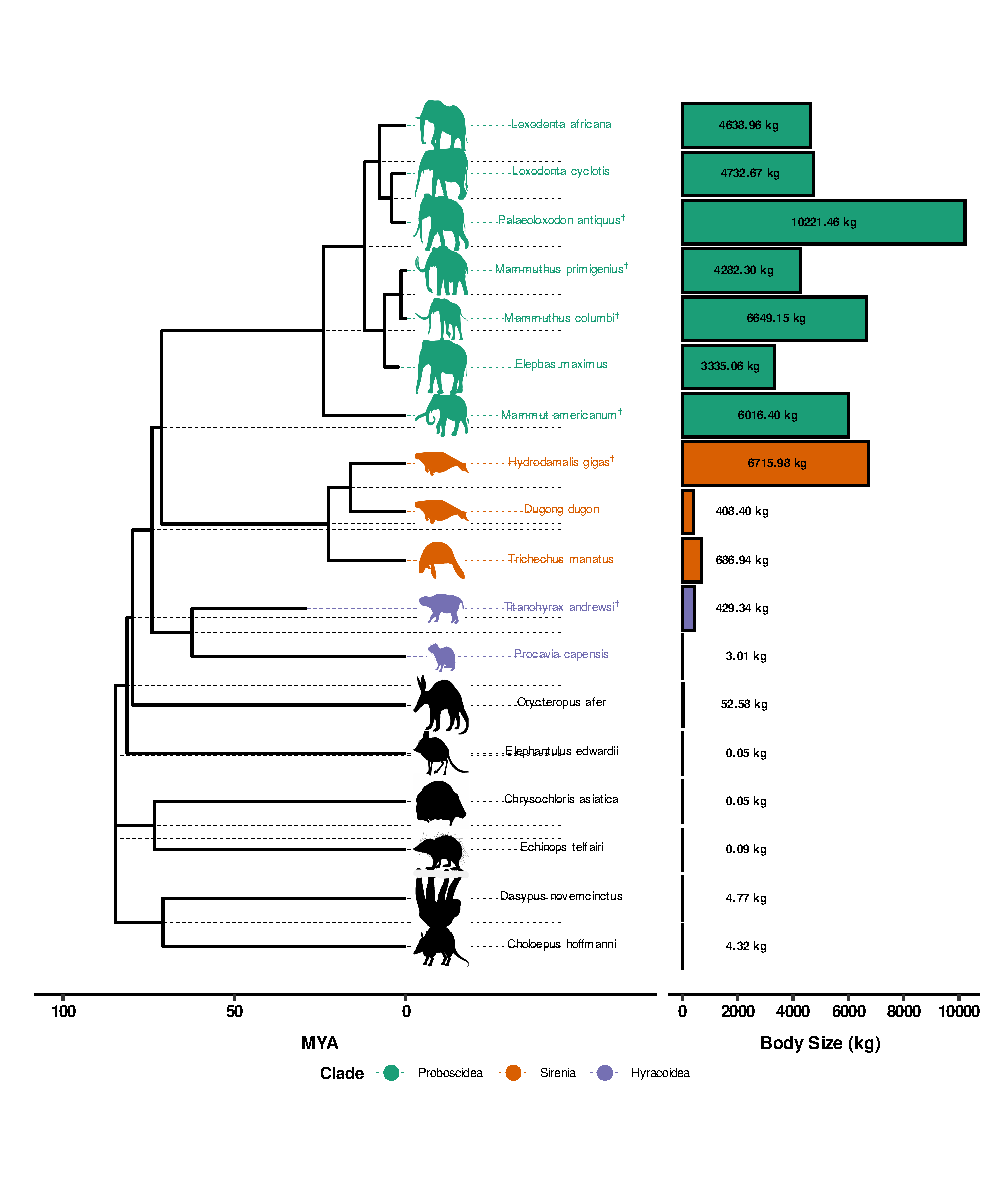
\includegraphics[width=6in,]{paper_PLOS_draft_files/figure-latex/Figure-intro-1} \caption{\emph{Atlantogenatans} with sequenced genomes, body sizes, and known lifespans {[}14,21{]}}\label{fig:Figure-intro}
\end{figure}

\begin{figure}[H]
\includegraphics[width=6in,]{paper_PLOS_draft_files/figure-latex/Figure-BodySize-1} \caption{Body sizes rapidly and frequently expand in Eutherians, especially in Atlantogenata. **A)** Tree of Eutherian species, colored by ln(Body Size) and with branch lengths set to the rate of change in body sizes, normalized by the square root of the root branch. Atlantogenata is highlighted at the bottom. **B)** Zoom-in of (**A**) on Atlantogenata. Silhuetes for the African Elephant, West Indian Manatee, Cape Elephant Shrew, Lesser Hedgehog Tenrec, Cape Golden Mole, Nine-Banded Armadillo, and Hoffman's Two-Toed Sloth are colored by their extant body sizes, while clade labels are colored based on the common ancestor's estimated body size. **C)** Confidence interval plot for representative species and ancestral nodes.}\label{fig:Figure-BodySize}
\end{figure}



\begin{figure}[H]
\includegraphics[width=6in,]{paper_PLOS_draft_files/figure-latex/Figure-CancerSuscept-1} \caption{Cancer succecptibility across \emph{Atlantogenata.} Branch lengths are set to the magnitude of change in cancer succeptiblity; colors indicate the magnitude and direction of the change.}\label{fig:Figure-CancerSuscept}
\end{figure}



\begin{figure}[H]
\includegraphics[width=6in,height=6in,]{paper_PLOS_draft_files/figure-latex/Figure-GeneDup-Cladogram-1} \caption{Gene duplications occur readily throughout \emph{Atlantogenata}. Shown here is a tree of \emph{Atlantogenatan} species with genomes, with the number of genes that underwent an increase in copy number overlayed at each node.}\label{fig:Figure-GeneDup-Cladogram}
\end{figure}



\begin{figure}[H]

{\centering \includegraphics[width=6in,height=6in,]{paper_PLOS_draft_files/figure-latex/Figure-GenomeCor-1} 

}

\caption{Correlations between genome quality metrics and ECNC metrics. Gene copy number metrics, and the genome quality metrics most strongly associated with them, are highlighted in red.}\label{fig:Figure-GenomeCor}
\end{figure}



\begin{figure}[H]
\includegraphics[width=6in,height=4in,]{paper_PLOS_draft_files/figure-latex/Figure-loxAfrORA-1} \caption{Overrepresentation Analysis of Duplicated Genes in Atlantogenata using Reactome Pathways.}\label{fig:Figure-loxAfrORA}
\end{figure}



\begin{figure}[H]
\includegraphics[width=6in,]{paper_PLOS_draft_files/figure-latex/Figure-loxAfrTP53-1} \caption{TP53-related genes are also duplicated and functional in \emph{Loxodonta africana}. \textbf{A)} Cladogram of \emph{Atlantogenata} highlighting along each branch when duplications for each gene occured. \textbf{B)} Gene expression data collected from pulically-available RNA-seq data for each duplicate in \textbf{A)}.}\label{fig:Figure-loxAfrTP53}
\end{figure}

\hypertarget{tables}{%
\section{TABLES}\label{tables}}

\begin{longtable}[t]{lrrrr}
\caption{\label{tab:Table-BodySize}Body Size and Confidence Intervals in Atlantogenata estimated using StableTraits.}\\
\toprule
Node & Size (log(g)) & 95\% CI (Low) & 95\% CI (High) & Rate (sqrt)\\
\midrule
\endfirsthead
\caption[]{\label{tab:Table-BodySize}Body Size and Confidence Intervals in Atlantogenata estimated using StableTraits. \textit{(continued)}}\\
\toprule
Node & Size (log(g)) & 95\% CI (Low) & 95\% CI (High) & Rate (sqrt)\\
\midrule
\endhead
\
\endfoot
\bottomrule
\endlastfoot
Cryptochloris wintoni & 3.13 & 3.13 & 3.13 & 5.78\\
Amblysomus marleyi & 3.53 & 3.53 & 3.53 & 3.79\\
Elephantulus revoili & 3.48 & 3.48 & 3.48 & 1.10\\
Titanohyrax andrewsi & 12.97 & 12.97 & 12.97 & 0.07\\
Titanohyrax ultimus & 14.08 & 14.08 & 14.08 & 34.61\\
\addlinespace
Megalohyrax sp  nov & 12.52 & 12.52 & 12.52 & 7.21\\
Elephas maximus asurus & 15.66 & 15.66 & 15.66 & 0.34\\
Protenrec tricuspis & 1.14 & 1.14 & 1.14 & 69.75\\
Microgale parvula & 1.16 & 1.16 & 1.16 & 33.46\\
Microgale pusilla & 1.25 & 1.25 & 1.25 & 34.31\\
\addlinespace
Geogale aurita & 1.90 & 1.90 & 1.90 & 40.07\\
Microgale longicaudata & 2.09 & 2.09 & 2.09 & 0.77\\
Microgale brevicaudata & 2.19 & 2.19 & 2.19 & 0.60\\
Microgale jobihely & 2.30 & 2.30 & 2.30 & 1.07\\
Microgale principula & 2.32 & 2.32 & 2.32 & 0.17\\
\addlinespace
Dilambdogale gheerbranti & 2.38 & 2.38 & 2.38 & 2.21\\
Microgale taiva & 2.47 & 2.47 & 2.47 & 0.13\\
Microgale cowani & 2.62 & 2.62 & 2.62 & 0.57\\
Eremitalpa granti & 3.14 & 3.14 & 3.14 & 9.65\\
Calcochloris obtusirostris & 3.27 & 3.27 & 3.27 & 13.38\\
\addlinespace
Neamblysomus julianae & 3.33 & 3.33 & 3.33 & 5.72\\
Chlorotalpa duthieae & 3.38 & 3.38 & 3.38 & 0.32\\
Chlorotalpa sclateri & 3.54 & 3.54 & 3.54 & 0.09\\
Macroscelides proboscideus & 3.64 & 3.64 & 3.64 & 14.17\\
Chrysochloris stuhlmanni & 3.74 & 3.74 & 3.74 & 0.33\\
\addlinespace
Oryzorictes hova & 3.79 & 3.79 & 3.79 & 22.77\\
Elephantulus myurus & 3.81 & 3.81 & 3.81 & 0.95\\
Elephantulus brachyrhynchus & 3.81 & 3.81 & 3.81 & 0.93\\
Elephantulus rozeti & 3.81 & 3.81 & 3.81 & 10.51\\
Elephantulus fuscus & 3.82 & 3.82 & 3.82 & 0.68\\
\addlinespace
Elephantulus intufi & 3.82 & 3.82 & 3.82 & 1.15\\
Microgale talazaci & 3.88 & 3.88 & 3.88 & 61.40\\
Chrysochloris asiatica & 3.89 & 3.89 & 3.89 & 3.34\\
Elephantulus edwardii & 3.90 & 3.90 & 3.90 & 0.24\\
Carpitalpa arendsi & 3.94 & 3.94 & 3.94 & 0.45\\
\addlinespace
Amblysomus corriae & 3.94 & 3.94 & 3.94 & 0.98\\
Amblysomus hottentotus & 3.98 & 3.98 & 3.98 & 0.02\\
Elephantulus fuscipes & 4.04 & 4.04 & 4.04 & 1.93\\
Elephantulus rufescens & 4.05 & 4.05 & 4.05 & 0.12\\
Neamblysomus gunningi & 4.09 & 4.09 & 4.09 & 3.26\\
\addlinespace
Elephantulus rupestris & 4.12 & 4.12 & 4.12 & 0.32\\
Amblysomus septentrionalis & 4.23 & 4.23 & 4.23 & 0.52\\
Chambius kasserinensis & 4.27 & 4.27 & 4.27 & 11.84\\
Amblysomus robustus & 4.33 & 4.33 & 4.33 & 1.38\\
Micropotamogale lamottei & 4.36 & 4.36 & 4.36 & 2.82\\
\addlinespace
Echinops telfairi & 4.47 & 4.47 & 4.47 & 7.75\\
Limnogale mergulus & 4.52 & 4.52 & 4.52 & 121.95\\
Hemicentetes semispinosus & 4.75 & 4.75 & 4.75 & 4.68\\
Chrysospalax villosus & 4.77 & 4.77 & 4.77 & 0.13\\
Petrodromus tetradactylus & 5.29 & 5.29 & 5.29 & 24.61\\
\addlinespace
Herodotius pattersoni & 5.50 & 5.50 & 5.50 & 11.64\\
Setifer setosus & 5.61 & 5.61 & 5.61 & 12.52\\
Rhynchocyon cirnei & 5.86 & 5.86 & 5.86 & 3.30\\
Metoldobotes sp  nov & 5.93 & 5.93 & 5.93 & 15.94\\
Chrysospalax trevelyani & 6.13 & 6.13 & 6.13 & 62.84\\
\addlinespace
Rhynchocyon petersi & 6.15 & 6.15 & 6.15 & 2.13\\
Rhynchocyon chrysopygus & 6.28 & 6.28 & 6.28 & 0.40\\
Potamogale velox & 6.49 & 6.49 & 6.49 & 103.04\\
Rhynchocyon udzungwensis & 6.57 & 6.57 & 6.57 & 4.33\\
Tenrec ecaudatus & 6.75 & 6.75 & 6.75 & 79.50\\
\addlinespace
Dasypus sabanicola & 7.05 & 7.05 & 7.05 & 12.18\\
Tolypeutes matacus & 7.11 & 7.11 & 7.11 & 15.96\\
Dasypus septemcinctus & 7.30 & 7.30 & 7.30 & 4.44\\
Zaedyus pichiy & 7.31 & 7.31 & 7.31 & 5.54\\
Dasypus hybridus & 7.31 & 7.31 & 7.31 & 4.05\\
\addlinespace
Chaetophractus villosus & 7.61 & 7.61 & 7.61 & 0.42\\
Chaetophractus nationi & 7.67 & 7.67 & 7.67 & 0.09\\
Heterohyrax brucei & 7.78 & 7.78 & 7.78 & 1.64\\
Cabassous centralis & 7.92 & 7.92 & 7.92 & 0.25\\
Seggeurius amourensis & 7.98 & 7.98 & 7.98 & 2.82\\
\addlinespace
Procavia capensis & 8.01 & 8.01 & 8.01 & 0.00\\
Dendrohyrax dorsalis & 8.06 & 8.06 & 8.06 & 1.86\\
Microhyrax lavocati & 8.13 & 8.13 & 8.13 & 0.73\\
Bradypus tridactylus & 8.23 & 8.23 & 8.23 & 0.48\\
Bradypus torquatus & 8.27 & 8.27 & 8.27 & 0.03\\
\addlinespace
Dasypus novemcinctus & 8.37 & 8.37 & 8.37 & 14.73\\
Euphractus sexcinctus & 8.43 & 8.43 & 8.43 & 14.99\\
Choloepus hoffmanni & 8.47 & 8.47 & 8.47 & 0.32\\
Bradypus variegatus & 8.49 & 8.49 & 8.49 & 0.51\\
Tamandua tetradactyla & 8.52 & 8.52 & 8.52 & 10.44\\
\addlinespace
Cyclopes didactylus & 8.53 & 8.53 & 8.53 & 2.15\\
Choloepus didactylus & 8.71 & 8.71 & 8.71 & 0.64\\
Thyrohyrax meyeri & 8.78 & 8.78 & 8.78 & 3.55\\
Saghatherium bowni & 9.13 & 9.13 & 9.13 & 15.85\\
Dasypus kappleri & 9.23 & 9.23 & 9.23 & 74.13\\
\addlinespace
Thyrohyrax domorictus & 9.30 & 9.30 & 9.30 & 1.15\\
Dimaitherium patnaiki & 9.57 & 9.57 & 9.57 & 18.23\\
Phosphatherium escuilliei & 9.62 & 9.62 & 9.62 & 326.23\\
Saghatherium antiquum & 9.73 & 9.73 & 9.73 & 2.90\\
Thyrohyrax litholagus & 10.01 & 10.01 & 10.01 & 28.58\\
\addlinespace
Myrmecophaga tridactyla & 10.26 & 10.26 & 10.26 & 41.03\\
Myorycteropus africanus & 10.27 & 10.27 & 10.27 & 0.57\\
Selenohyrax chatrathi & 10.73 & 10.73 & 10.73 & 14.99\\
Priodontes maximus & 10.82 & 10.82 & 10.82 & 268.43\\
Orycteropus afer & 10.87 & 10.87 & 10.87 & 6.59\\
\addlinespace
Antilohyrax pectidens & 10.93 & 10.93 & 10.93 & 13.69\\
Bunohyrax fajumensis & 11.32 & 11.32 & 11.32 & 1.45\\
Afrohyrax championi & 11.32 & 11.32 & 11.32 & 0.19\\
Geniohyus mirus & 11.33 & 11.33 & 11.33 & 5.44\\
Prorastomus sirenoides & 11.49 & 11.49 & 11.49 & 13.61\\
\addlinespace
Elephas antiquus falconeri & 11.51 & 11.51 & 11.51 & 6.12\\
Pachyhyrax crassidentatus & 11.81 & 11.81 & 11.81 & 2.29\\
Megalohyrax eocaenus & 11.95 & 11.95 & 11.95 & 0.24\\
Elephas cypriotes & 12.21 & 12.21 & 12.21 & 1.90\\
Bunohyrax major & 12.36 & 12.36 & 12.36 & 11.39\\
\addlinespace
Titanohyrax angustidens & 12.48 & 12.48 & 12.48 & 0.04\\
Daouitherium rebouli & 12.80 & 12.80 & 12.80 & 0.74\\
Arcanotherium savagei & 12.89 & 12.89 & 12.89 & 7.29\\
Dugong dugon & 12.92 & 12.92 & 12.92 & 5.85\\
Trichechus senegalensis & 13.03 & 13.03 & 13.03 & 0.57\\
\addlinespace
Trichechus inunguis & 13.08 & 13.08 & 13.08 & 0.69\\
Protosiren smithae & 13.20 & 13.20 & 13.20 & 33.69\\
Numidotherium koholense & 13.23 & 13.23 & 13.23 & 2.29\\
Omanitherium dhofarensis & 13.35 & 13.35 & 13.35 & 0.03\\
Trichechus manatus & 13.44 & 13.44 & 13.44 & 1.39\\
\addlinespace
Moeritherium spp & 13.82 & 13.82 & 13.82 & 5.71\\
Phiomia spp & 13.89 & 13.89 & 13.89 & 3.64\\
Elephas maximus & 15.02 & 15.02 & 15.02 & 5.81\\
Barytherium spp & 15.20 & 15.20 & 15.20 & 73.58\\
Mammuthus primigenius & 15.27 & 15.27 & 15.27 & 2.17\\
\addlinespace
Mammut borsoni & 16.49 & 16.49 & 16.49 & 15.33\\
Mammuthus trogontherii & 16.38 & 16.38 & 16.38 & 16.00\\
Loxodonta africana & 15.35 & 15.35 & 15.35 & 1.28\\
Loxodonta cyclotis & 15.37 & 15.37 & 15.37 & 3.72\\
Palaeoloxodon antiquus & 16.14 & 16.14 & 16.14 & 0.01\\
\addlinespace
Palaeoloxodon namadicus & 16.81 & 16.81 & 16.81 & 12.81\\
Mammut americanum & 15.61 & 15.61 & 15.61 & 0.95\\
Mammuthus columbi & 15.71 & 15.71 & 15.71 & 0.91\\
Hydrodamalis gigas & 15.72 & 15.72 & 15.72 & 172.52\\
Atlantogenata & 5.55 & 4.06 & 7.95 & 0.03\\
\addlinespace
Afrotheria & 5.55 & 4.05 & 7.96 & 0.00\\
Afrosoricida & 4.35 & 2.58 & 6.13 & 44.49\\
Macroscelidae & 5.27 & 3.98 & 6.85 & 2.49\\
Pseudoungulata & 9.76 & 5.21 & 12.78 & 545.83\\
Paenungulata & 10.13 & 7.24 & 13.02 & 4.42\\
\addlinespace
Tethytheria & 12.60 & 10.25 & 13.81 & 187.47\\
Proboscidea & 15.23 & 14.22 & 16.24 & 30.28\\
Elephantidae & 15.49 & 14.89 & 16.10 & 2.21\\
Elephantina & 15.51 & 15.08 & 15.96 & 0.01\\
Mammuthus & 15.54 & 15.24 & 15.85 & 0.47\\
\addlinespace
Loxodontini & 15.55 & 15.02 & 16.11 & 0.11\\
Loxodona & 15.72 & 15.16 & 16.30 & 0.86\\
Xenarthra & 7.57 & 5.96 & 9.18 & 124.94\\*
\end{longtable}

\begin{table}

\caption{\label{tab:Table-CancerSuscept}Estimated Cancer Succeptibilty for nodes in Atlantogenata}
\centering
\resizebox{\linewidth}{!}{
\begin{tabular}[t]{lrlllr}
\toprule
Node & Est. Lifespan & K1 & K2 & Change in K & log2 Change\\
\midrule
Loxodontini & 34.38 & 1.47e+16 & 2.97e+15 & 4.94e+00 & 2.31\\
Loxodonta africana & 65.00 & 2.47e+17 & 1.47e+16 & 1.68e+01 & 4.07\\
Loxodona & 34.38 & 1.47e+16 & 1.47e+16 & 1.00e+00 & 0.00\\
Loxodonta cyclotis & 31.12 & 2.97e+15 & 1.47e+16 & 2.02e-01 & -2.31\\
Palaeoloxodon antiquus & 34.38 & 1.47e+16 & 1.47e+16 & 1.00e+00 & 0.00\\
\addlinespace
Elephantidae & 31.12 & 2.97e+15 & 1.40e+07 & 2.13e+08 & 27.66\\
Elephantina & 34.38 & 1.47e+16 & 2.97e+15 & 4.94e+00 & 2.31\\
Elephas maximus & 65.50 & 2.58e+17 & 1.47e+16 & 1.76e+01 & 4.14\\
Mammuthus & 34.38 & 1.47e+16 & 1.47e+16 & 1.00e+00 & 0.00\\
Mammuthus primigenius & 31.12 & 2.97e+15 & 1.47e+16 & 2.02e-01 & -2.31\\
\addlinespace
Mammuthus columbi & 34.38 & 1.47e+16 & 1.47e+16 & 1.00e+00 & 0.00\\
Proboscidea & 9.41 & 1.40e+07 & 1.21e+14 & 1.15e-07 & -23.05\\
Mammut americanum & 34.38 & 1.47e+16 & 1.40e+07 & 1.05e+09 & 29.97\\
Tethytheria & 25.49 & 1.21e+14 & 1.01e+12 & 1.21e+02 & 6.92\\
Trichechus manatus & 69.00 & 4.77e+16 & 1.21e+14 & 3.93e+02 & 8.62\\
\addlinespace
Paenungulata & 18.91 & 1.01e+12 & 1.01e+12 & 1.00e+00 & 0.00\\
Procavia capensis & 14.80 & 3.13e+10 & 1.01e+12 & 3.11e-02 & -5.01\\
Pseudoungulata & 18.91 & 1.01e+12 & 1.69e+09 & 5.97e+02 & 9.22\\
Orycteropus afer & 29.80 & 4.19e+13 & 1.01e+12 & 4.17e+01 & 5.38\\
Elephantulus edwardii & 10.40 & 6.90e+07 & 1.69e+09 & 4.09e-02 & -4.61\\
\addlinespace
Afrosoricida & 10.40 & 6.90e+07 & 1.69e+09 & 4.09e-02 & -4.61\\
Chrysochloris asiatica & 10.40 & 6.90e+07 & 6.90e+07 & 1.00e+00 & 0.00\\
Echinops telfairi & 19.00 & 2.57e+09 & 6.90e+07 & 3.72e+01 & 5.22\\
Afrotheria & 12.69 & 1.69e+09 & 2.83e+06 & 5.97e+02 & 9.22\\
Xenarthra & 20.89 & 4.97e+12 & 2.83e+06 & 1.76e+06 & 20.75\\
\addlinespace
Dasypus novemcinctus & 22.30 & 3.67e+11 & 4.97e+12 & 7.37e-02 & -3.76\\
Choloepus hoffmanni & 41.00 & 1.42e+13 & 4.97e+12 & 2.85e+00 & 1.51\\
Atlantogenata & 8.52 & 2.83e+06 & 2.83e+06 & 1.00e+00 & 0.00\\
Afroinsectivora & 12.69 & 1.69e+09 & 1.69e+09 & 1.00e+00 & 0.00\\
\bottomrule
\end{tabular}}
\end{table}

\begin{table}

\caption{\label{tab:Table-GeneDup}Summary of duplications in Atlantogenata}
\centering
\resizebox{\linewidth}{!}{
\begin{tabular}[t]{lllrrllr}
\toprule
Species & Common Name & Size (g) & \#Hits & \#Duplicated & \% Genes Found & \% Hits Duplicated & Mean ECNC/Hit\\
\midrule
Choloepus hoffmanni & Hoffmans Two-Toed Sloth & 4.3e+03 & 14082 & 3204 & 78.19\% & 22.75\% & 0.98\\
Chrysochloris asiatica & Cape Golden Mole & 49 & 13547 & 2716 & 75.22\% & 20.05\% & 0.99\\
Dasypus novemcinctus & Nine-Banded Armadillo & 4.8e+03 & 13819 & 2605 & 76.73\% & 18.85\% & 0.98\\
Echinops telfairi & Lesser Hedgehog Tenrec & 87 & 12903 & 1670 & 71.64\% & 12.94\% & 0.99\\
Elephantulus edwardii & Cape Elephant Shrew & 49 & 12884 & 3048 & 71.53\% & 23.66\% & 0.99\\
\addlinespace
Elephas maximus & Asian Elephant & 3.3e+06 & 14073 & 907 & 78.14\% & 6.44\% & 1.00\\
Loxodonta africana & African Savanna Elephant & 4.6e+06 & 14051 & 940 & 78.01\% & 6.69\% & 1.00\\
Loxodonta cyclotis & African Forest Elephant & 4.7e+06 & 14065 & 900 & 78.09\% & 6.40\% & 1.00\\
Mammut americanum & American Mastodon & 6e+06 & 13840 & 737 & 76.84\% & 5.33\% & 1.00\\
Mammuthus columbi & Columbian Mammoth & 6.6e+06 & 13059 & 426 & 72.51\% & 3.26\% & 1.00\\
\addlinespace
Mammuthus primigenius & Woolly Mammoth & 4.3e+06 & 13935 & 723 & 77.37\% & 5.19\% & 1.00\\
Orycteropus afer & Aardvark & 5.3e+04 & 13880 & 1083 & 77.06\% & 7.80\% & 0.99\\
Palaeoloxodon antiquus & Straight Tusked Elephant & 1e+07 & 13969 & 745 & 77.56\% & 5.33\% & 1.00\\
Procavia capensis & Rock Hyrax & 3e+03 & 13672 & 788 & 75.91\% & 5.76\% & 1.00\\
Trichechus manatus & Manatee & 6.9e+05 & 14092 & 1046 & 78.24\% & 7.42\% & 1.00\\
\bottomrule
\end{tabular}}
\end{table}

\begin{table}

\caption{\label{tab:Table-ORAFreqDatabase}Number of pathways overrepresented among duplicated genes at different FDRs.}
\centering
\resizebox{\linewidth}{!}{
\begin{tabular}[t]{llrrrr}
\toprule
Ancestor & Node & Pathways at FDR<0.1 & Pathways at FDR<0.2 & Pathways at FDR<0.3 & Pathways at FDR<0.5\\
\midrule
Afroinsectivora & Elephantulus edwardii & 252 & 37 & 30 & 87\\
Afrosoricida & Chrysochloris asiatica & 90 & 48 & 43 & 105\\
Afrosoricida & Echinops telfairi & 0 & 2 & 0 & 31\\
Afrotheria & Afroinsectivora & 0 & 0 & 0 & 33\\
Loxodontini & Loxodonta africana & 6 & 0 & 1 & 0\\
\addlinespace
Paenungulata & Tethytheria & 0 & 0 & 0 & 2\\
Proboscidea & Mammut americanum & 0 & 0 & 0 & 6\\
Pseudoungulata & Orycteropus afer & 27 & 67 & 29 & 67\\
Tethytheria & Proboscidea & 0 & 3 & 0 & 3\\
Tethytheria & Trichechus manatus & 4 & 0 & 0 & 2\\
\bottomrule
\end{tabular}}
\end{table}

\begin{table}

\caption{\label{tab:Table-SRAData}NCBI SRA datasets used in this study, along with key biological and genome information.}
\centering
\resizebox{\linewidth}{!}{
\begin{tabular}[t]{lll>{\raggedright\arraybackslash}p{10em}>{\raggedright\arraybackslash}p{10em}}
\toprule
Organism & Common Name & Genome & SRA Acc. & Tissues\\
\midrule
Dasypus novemcinctus & Nine-banded armadillo & dasNov3 & SRR494779, SRR494767, SRR494780, SRR494770, SRR309130, SRR494771, SRR4043756, SRR494776, SRR494778, SRR4043762, SRR4043755, SRR6206923, SRR4043761, SRR4043760, SRR6206913, SRR4043763, SRR494772, SRR494781, SRR494774, SRR494777, SRR494775, SRR4043754, SRR1289524, SRR4043758, SRR6206903, SRR1289523, SRR4043759, SRR3222425, SRR494768, SRR494769, SRR6206908, SRR4043757, SRR494766, SRR6206918, SRR494773 & Kidney, Spleen, Cerebellum W/ Brainstem, Rt. Quadricep, Mid-Stage Pregnant Endometrium, Cervix, Lung, Liver, Skeletal Muscle, Ascending Colon, Pregnant Armadillo Endometrium, Heart, Placenta\\
Loxodonta africana & African savanna elephant & loxAfr3, loxAfrC, loxAfr4 & SRR6307198, SRR1041765, SRR6307199, SRR6307201, SRR6307196, SRR6307202, SRR6307200, SRR6307195, SRR975188, SRR6307194, SRR6307204, SRR3222430, SRR6307205, SRR975189, SRR6307197, SRR6307203 & Blood, Fibroblast, Placenta\\
Trichechus manatus latirostris & Manatee & triMan1, triManLat2 & SRR4228542, SRR4228545, SRR4228544, SRR4228539, SRR4228541, SRR4228538, SRR4228546, SRR4228537, SRR4228540, SRR4228543, SRR4228547 & Buffy Coat\\
\bottomrule
\end{tabular}}
\end{table}

\begin{table}

\caption{\label{tab:Table-Genomes}Genomes used in this study.}
\centering
\resizebox{\linewidth}{!}{
\begin{tabular}[t]{lllll}
\toprule
Species & Common Name & Genomes & Highest Quality Genome & Citation\\
\midrule
Choloepus hoffmanni & Hoffmans two-toed sloth & choHof1, choHof2, choHof-C\_hoffmanni-2.0.1\_HiC & choHof-C\_hoffmanni-2.0.1\_HiC & NA\\
Chrysochloris asiatica & Cape golden mole & chrAsi1m & chrAsi1m & NA\\
Dasypus novemcinctus & Nine-banded armadillo & dasNov3 & dasNov3 & NA\\
Echinops telfairi & Lesser Hedgehog Tenrec & echTel2 & echTel2 & NA\\
Elephantulus edwardii & Cape elephant shrew & eleEdw1m & eleEdw1m & NA\\
\addlinespace
Elephas maximus & Asian elephant & eleMaxD & eleMaxD & NA\\
Loxodonta africana & African savanna elephant & loxAfr3, loxAfrC, loxAfr4 & loxAfr4 & NA\\
Loxodonta cyclotis & African forest elephant & loxCycF & loxCycF & NA\\
Mammut americanum & American mastodon & mamAmeI & mamAmeI & NA\\
Mammuthus columbi & Columbian mammoth & mamColU & mamColU & NA\\
\addlinespace
Mammuthus primigenius & Woolly mammoth & mamPriV & mamPriV & NA\\
Orycteropus afer & Aardvark & oryAfe1, oryAfe2 & oryAfe2 & NA\\
Palaeoloxodon antiquus & Straight tusked elephant & palAntN & palAntN & NA\\
Procavia capensis & Rock hyrax & proCap1, proCap2, proCap-Pcap\_2.0\_HiC & proCap-Pcap\_2.0\_HiC & NA\\
Trichechus manatus latirostris & Manatee & triMan1, triManLat2 & triManLat2 & NA\\
\bottomrule
\end{tabular}}
\end{table}

\hypertarget{supplementary-figures}{%
\section{SUPPLEMENTARY FIGURES}\label{supplementary-figures}}



\begin{figure}[H]
\includegraphics[width=6in,]{paper_PLOS_draft_files/figure-latex/Figure-ECNC-1} \caption{Estimated Copy Number by Coverage (ECNC) consolidates fragmented genes while accounting for missing domains in homologs. \textbf{A)} A single, contiguous gene homolog in a target genome with 100\% query length coverage has an ECNC of 1.0. \textbf{B)} Two contiguous gene homologs, each with 100\% query length coverage have an ECNC of 2.0. \textbf{C)} A single gene homolog, split across multiple scaffolds and contigs in a fragmented target genome; BLAT identifies each fragment as a single hit. Per nucleotide of query sequence, there is only one corresponding nucleotide over all the hits, thus the ECNC is 1.0. \textbf{D)} Two gene homologs, one fragmented and one contiguous. 100\% of nucleotides in the query sequence are represented between all hits; however, every nucleotide in the query has two matching nucleotides in the target genome, thus the ECNC is 2.0. \textbf{E)} One true gene homolog in the target genome, plus multiple hits of a conserved domain that span 20\% of the query sequence. While 100\% of the query sequence is represented in total, 20\% of the nucleotides have 4 hits. Thus, the ECNC for this gene is 1.45. \textbf{F)} Two real gene homologs; one hit is contiguous, one hit is fragmented in two, and the tail end of both sequences was not identified by BLAT due to sequence divergence. Only 75\% of the query sequence was covered in total between the hits, but for that 75\%, each nucleotide has two hits. As such, ECNC is equal to 2.0 for this gene.}\label{fig:Figure-ECNC}
\end{figure}

\begin{figure}[H]
\includegraphics[width=6in,]{paper_PLOS_draft_files/figure-latex/Figure-GeneDup-BLScaled-1} \caption{Gene copy increases polarized along Atlantogenata, colored by ln(Body Size), with branch lengths equal to the change in gene copy number}\label{fig:Figure-GeneDup-BLScaled}
\end{figure}

\begin{verbatim}
## Warning: TODO: Make HQ version of this figure
\end{verbatim}

\begin{figure}[H]
\includegraphics[width=6in,]{paper_PLOS_draft_files/figure-latex/Figure-RBHBStrategy-1} \caption{Full version of RecBlat strategy, but low quality}\label{fig:Figure-RBHBStrategy}
\end{figure}

\begin{figure}[H]
\includegraphics[width=6in,]{paper_PLOS_draft_files/figure-latex/Figure-TimeTree-Eutheria-1} \caption{The time-calibrated Eutherian tree used as input for StableTraits, from Bininda-Emonds et al and Puttick and Thomas}\label{fig:Figure-TimeTree-Eutheria}
\end{figure}

\hypertarget{references}{%
\section*{References}\label{references}}
\addcontentsline{toc}{section}{References}

\hypertarget{refs}{}
\leavevmode\hypertarget{ref-Savage2007}{}%
1. Savage VM, Allen AP, Brown JH, Gillooly JF, Herman AB, Woodruff WH, et al. Scaling of number, size, and metabolic rate of cells with body size in mammals. Proceedings of the National Academy of Sciences. 2007;104: 4718--4723. doi:\href{https://doi.org/10.1073/pnas.0611235104}{10.1073/pnas.0611235104}

\leavevmode\hypertarget{ref-Green2011}{}%
2. Green J, Cairns BJ, Casabonne D, Wright FL, Reeves G, Beral V, et al. Height and cancer incidence in the Million Women Study: prospective cohort, and meta-analysis of prospective studies of height and total cancer risk. The Lancet Oncology. 2011;12: 785--794. doi:\href{https://doi.org/10.1016/s1470-2045(11)70154-1}{10.1016/s1470-2045(11)70154-1}

\leavevmode\hypertarget{ref-Nunney:20181c2}{}%
3. Nunney L. Size matters: height, cell number and a person's risk of cancer. Proc R Soc B. 2018;285: 20181743. doi:\href{https://doi.org/10.1098/rspb.2018.1743}{10.1098/rspb.2018.1743}

\leavevmode\hypertarget{ref-Dobson2013}{}%
4. Dobson JM. Breed-predispositions to cancer in pedigree dogs. ISRN veterinary science. 2013;2013: 941275. doi:\href{https://doi.org/10.1155/2013/941275}{10.1155/2013/941275}

\leavevmode\hypertarget{ref-Dorn1968}{}%
5. Dorn CR, Taylor DON, Schneider R, Hibbard HH, Klauber MR. Survey of Animal Neoplasms in Alameda and Contra Costa Counties, California. II. Cancer Morbidity in Dogs and Cats From Alameda County\textless{}xref ref-type="fn" rid="FN2"\textgreater{}2\textless{}/xref\textgreater{}. JNCI: Journal of the National Cancer Institute. 1968;40: 307--318. doi:\href{https://doi.org/10.1093/jnci/40.2.307}{10.1093/jnci/40.2.307}

\leavevmode\hypertarget{ref-Caulin2011}{}%
6. Caulin AF, Maley CC. Peto's Paradox: evolution's prescription for cancer prevention. Trends in ecology \& evolution. 2011;26: 175--82. doi:\href{https://doi.org/10.1016/j.tree.2011.01.002}{10.1016/j.tree.2011.01.002}

\leavevmode\hypertarget{ref-Leroi2003}{}%
7. Leroi AM, Koufopanou V, Burt A. Cancer selection. Nature Reviews Cancer. 2003;3: 226--231. doi:\href{https://doi.org/10.1038/nrc1016}{10.1038/nrc1016}

\leavevmode\hypertarget{ref-Peto1975}{}%
8. Peto R, Roe F, Lee P, Levy L, Clack J. Cancer and ageing in mice and men. British Journal of Cancer. 1975;32: 411--426. doi:\href{https://doi.org/10.1038/bjc.1975.242}{10.1038/bjc.1975.242}

\leavevmode\hypertarget{ref-Ashur-Fabian2004}{}%
9. Ashur-Fabian O, Avivi A, Trakhtenbrot L, Adamsky K, Cohen M, Kajakaro G, et al. Evolution of p53 in hypoxia-stressed Spalax mimics human tumor mutation. Proceedings of the National Academy of Sciences. 2004;101: 12236--12241. doi:\href{https://doi.org/10.1073/pnas.0404998101}{10.1073/pnas.0404998101}

\leavevmode\hypertarget{ref-Seluanov2008}{}%
10. Seluanov A, Hine C, Bozzella M, Hall A, Sasahara THC, Ribeiro AACM, et al. Distinct tumor suppressor mechanisms evolve in rodent species that differ in size and lifespan. Aging cell. 2008;7: 813--23. doi:\href{https://doi.org/10.1111/j.1474-9726.2008.00431.x}{10.1111/j.1474-9726.2008.00431.x}

\leavevmode\hypertarget{ref-Gorbunova2012}{}%
11. Gorbunova V, Hine C, Tian X, Ablaeva J, Gudkov AV, Nevo E, et al. Cancer resistance in the blind mole rat is mediated by concerted necrotic cell death mechanism. Proceedings of the National Academy of Sciences of the United States of America. 2012;109: 19392--6. doi:\href{https://doi.org/10.1073/pnas.1217211109}{10.1073/pnas.1217211109}

\leavevmode\hypertarget{ref-Tian2013}{}%
12. Tian X, Azpurua J, Hine C, Vaidya A, Myakishev-Rempel M, Ablaeva J, et al. High molecular weight hyaluronan mediates the cancer resistance of the naked mole-rat. 2013;499. doi:\href{https://doi.org/10.1038/nature12234}{10.1038/nature12234}

\leavevmode\hypertarget{ref-Sulak2015}{}%
13. Sulak M, Fong L, Mika K, Chigurupati S, Yon L, Mongan NP, et al. TP53 copy number expansion is associated with the evolution of increased body size and an enhanced DNA damage response in elephants. eLife. 2016;5: e11994. doi:\href{https://doi.org/10.7554/elife.11994}{10.7554/elife.11994}

\leavevmode\hypertarget{ref-HAGR}{}%
14. Tacutu R, Craig T, Budovsky A, Wuttke D, Lehmann G, Taranukha D, et al. Human Ageing Genomic Resources: Integrated databases and tools for the biology and genetics of ageing. Nucleic Acids Research. 2013;41: D1027--D1033. doi:\href{https://doi.org/10.1093/nar/gks1155}{10.1093/nar/gks1155}

\leavevmode\hypertarget{ref-Schwartz1995}{}%
15. Schwartz GT, Rasmussen DT, Smith RJ. Body-Size Diversity and Community Structure of Fossil Hyracoids. Journal of Mammalogy. 1995;76: 1088--1099. doi:\href{https://doi.org/10.2307/1382601}{10.2307/1382601}

\leavevmode\hypertarget{ref-Scheffer1972}{}%
16. Scheffer VB. The Weight of the Steller Sea Cow. Journal of Mammalogy. 1972;53: 912--914. doi:\href{https://doi.org/10.2307/1379236}{10.2307/1379236}

\leavevmode\hypertarget{ref-Larramendi:20151c2}{}%
17. Larramendi A. Shoulder Height, Body Mass, and Shape of Proboscideans. Acta Palaeontologica Polonica. 2015;61. doi:\href{https://doi.org/10.4202/app.00136.2014}{10.4202/app.00136.2014}

\leavevmode\hypertarget{ref-OLeary2013a}{}%
18. O'Leary MA, Bloch JI, Flynn JJ, Gaudin TJ, Giallombardo A, Giannini NP, et al. The placental mammal ancestor and the post-K-Pg radiation of placentals. Science (New York, NY). 2013;339: 662--7. doi:\href{https://doi.org/10.1126/science.1229237}{10.1126/science.1229237}

\leavevmode\hypertarget{ref-Springer2013}{}%
19. Springer MS, Meredith RW, Teeling EC, Murphy WJ. Technical comment on "The placental mammal ancestor and the post-K-Pg radiation of placentals". Science (New York, NY). 2013;341: 613. doi:\href{https://doi.org/10.1126/science.1238025}{10.1126/science.1238025}

\leavevmode\hypertarget{ref-OLeary2013b}{}%
20. O'Leary MA, Bloch JI, Flynn JJ, Gaudin TJ, Giallombardo A, Giannini NP, et al. Response to comment on "The placental mammal ancestor and the post-K-Pg radiation of placentals". Science (New York, NY). 2013;341: 613. doi:\href{https://doi.org/10.1126/science.1238162}{10.1126/science.1238162}

\leavevmode\hypertarget{ref-PuttickAndThomas2015}{}%
21. Puttick MN, Thomas GH. Fossils and living taxa agree on patterns of body mass evolution: a case study with Afrotheria. Proceedings Biological sciences / The Royal Society. 2015;282: 20152023. doi:\href{https://doi.org/10.1098/rspb.2015.2023}{10.1098/rspb.2015.2023}

\leavevmode\hypertarget{ref-Abegglen:JAMA2015}{}%
22. Abegglen LM, Caulin AF, Chan A, Lee K, Robinson R, Campbell MS, et al. Potential Mechanisms for Cancer Resistance in Elephants and Comparative Cellular Response to DNA Damage in Humans. JAMA. 2015;314: 1850--1860. doi:\href{https://doi.org/10.1001/jama.2015.13134}{10.1001/jama.2015.13134}

\leavevmode\hypertarget{ref-Vazquez2018}{}%
23. Vazquez JM, Sulak M, Chigurupati S, Lynch VJ. A Zombie LIF Gene in Elephants Is Upregulated by TP53 to Induce Apoptosis in Response to DNA Damage. Cell Reports. 2018;24: 1765--1776. doi:\href{https://doi.org/10.1016/j.celrep.2018.07.042}{10.1016/j.celrep.2018.07.042}

\leavevmode\hypertarget{ref-Caulin2015}{}%
24. Caulin AF, Graham TA, Wang L-S, Maley CC. Solutions to Peto's paradox revealed by mathematical modelling and cross-species cancer gene analysis. Philosophical transactions of the Royal Society of London Series B, Biological sciences. 2015;370: 20140222. doi:\href{https://doi.org/10.1098/rstb.2014.0222}{10.1098/rstb.2014.0222}

\leavevmode\hypertarget{ref-Doherty2016}{}%
25. Doherty A, Magalhães J de. Has gene duplication impacted the evolution of Eutherian longevity? Aging Cell. 2016;15: 978--980. doi:\href{https://doi.org/10.1111/acel.12503}{10.1111/acel.12503}

\leavevmode\hypertarget{ref-Bininda-Emonds2008}{}%
26. Bininda-Emonds ORP, Cardillo M, Jones KE, MacPhee RDE, Beck RMD, Grenyer R, et al. Erratum: The delayed rise of present-day mammals. Nature. 2008;456: 274--274. doi:\href{https://doi.org/10.1038/nature07347}{10.1038/nature07347}

\leavevmode\hypertarget{ref-ElliotAndMooers2014}{}%
27. Elliot MG, Mooers AØ. Inferring ancestral states without assuming neutrality or gradualism using a stable model of continuous character evolution. BMC evolutionary biology. 2014;14: 226. doi:\href{https://doi.org/10.1186/s12862-014-0226-8}{10.1186/s12862-014-0226-8}

\leavevmode\hypertarget{ref-blat}{}%
28. Kent JW. BLAT?The BLAST-Like Alignment Tool. Genome Research. 2002;12: 656--664. doi:\href{https://doi.org/10.1101/gr.229202}{10.1101/gr.229202}

\leavevmode\hypertarget{ref-AltenhoffAndDessimoz2009}{}%
29. Altenhoff AM, Dessimoz C. Phylogenetic and functional assessment of orthologs inference projects and methods. PLoS computational biology. 2009;5: e1000262. doi:\href{https://doi.org/10.1371/journal.pcbi.1000262}{10.1371/journal.pcbi.1000262}

\leavevmode\hypertarget{ref-SalichosAndRokas2011}{}%
30. Salichos L, Rokas A. Evaluating ortholog prediction algorithms in a yeast model clade. PloS one. 2011;6: e18755. doi:\href{https://doi.org/10.1371/journal.pone.0018755}{10.1371/journal.pone.0018755}

\leavevmode\hypertarget{ref-uniprot}{}%
31. Consortium TU. UniProt: the universal protein knowledgebase. Nucleic Acids Research. 2017;45: D158--D169. doi:\href{https://doi.org/10.1093/nar/gkw1099}{10.1093/nar/gkw1099}

\leavevmode\hypertarget{ref-gVolante}{}%
32. Nishimura O, Hara Y, Kuraku S. gVolante for standardizing completeness assessment of genome and transcriptome assemblies. Bioinformatics. 2017;33: 3635--3637. doi:\href{https://doi.org/10.1093/bioinformatics/btx445}{10.1093/bioinformatics/btx445}

\leavevmode\hypertarget{ref-CEGMA}{}%
33. Parra G, Bradnam K, Ning Z, Keane T, Korf I. Assessing the gene space in draft genomes. Nucleic Acids Research. 2008;37: 289--297. doi:\href{https://doi.org/10.1093/nar/gkn916}{10.1093/nar/gkn916}

\leavevmode\hypertarget{ref-HISAT}{}%
34. Kim D, Langmead B, Salzberg SL. HISAT: a fast spliced aligner with low memory requirements. Nature Methods. 2015;12: 357--360. doi:\href{https://doi.org/10.1038/nmeth.3317}{10.1038/nmeth.3317}

\leavevmode\hypertarget{ref-StringTie}{}%
35. Pertea M, Pertea GM, Antonescu CM, Chang T-C, Mendell JT, Salzberg SL. StringTie enables improved reconstruction of a transcriptome from RNA-seq reads. Nature Biotechnology. 2015;33: 290--295. doi:\href{https://doi.org/10.1038/nbt.3122}{10.1038/nbt.3122}

\leavevmode\hypertarget{ref-Tuxedo}{}%
36. Pertea M, Kim D, Pertea GM, Leek JT, Salzberg SL. Transcript-level expression analysis of RNA-seq experiments with HISAT, StringTie and Ballgown. Nature Protocols. 2016;11: 1650--1667. doi:\href{https://doi.org/10.1038/nprot.2016.095}{10.1038/nprot.2016.095}

\leavevmode\hypertarget{ref-IQTREE}{}%
37. Minh BQ, Schmidt HA, Chernomor O, Schrempf D, Woodhams MD, Haeseler A von, et al. IQ-TREE 2: New Models and Efficient Methods for Phylogenetic Inference in the Genomic Era. Molecular Biology and Evolution. 2020;37: 1530--1534. doi:\href{https://doi.org/10.1093/molbev/msaa015}{10.1093/molbev/msaa015}

\leavevmode\hypertarget{ref-UFBoot2}{}%
38. Hoang DT, Chernomor O, Haeseler A von, Minh BQ, Vinh LS. UFBoot2: Improving the Ultrafast Bootstrap Approximation. Molecular Biology and Evolution. 2017;35: 518--522. doi:\href{https://doi.org/10.1093/molbev/msx281}{10.1093/molbev/msx281}

\leavevmode\hypertarget{ref-ModelFinder}{}%
39. Kalyaanamoorthy S, Minh BQ, Wong TKF, Haeseler A von, Jermiin LS. ModelFinder: fast model selection for accurate phylogenetic estimates. Nature Methods. 2017;14: 587--589. doi:\href{https://doi.org/10.1038/nmeth.4285}{10.1038/nmeth.4285}

\leavevmode\hypertarget{ref-PMSF}{}%
40. Wang H-C, Minh BQ, Susko E, Roger AJ. Modeling Site Heterogeneity with Posterior Mean Site Frequency Profiles Accelerates Accurate Phylogenomic Estimation. Systematic Biology. 2017;67: 216--235. doi:\href{https://doi.org/10.1093/sysbio/syx068}{10.1093/sysbio/syx068}

\leavevmode\hypertarget{ref-Schrempf2019}{}%
41. Schrempf D, Minh BQ, Haeseler A von, Kosiol C. Polymorphism-Aware Species Trees with Advanced Mutation Models, Bootstrap, and Rate Heterogeneity. Molecular Biology and Evolution. 2019;36: 1294--1301. doi:\href{https://doi.org/10.1093/molbev/msz043}{10.1093/molbev/msz043}

\leavevmode\hypertarget{ref-Soubrier2012}{}%
42. Soubrier J, Steel M, Lee MSY, Sarkissian CD, Guindon S, Ho SYW, et al. The Influence of Rate Heterogeneity among Sites on the Time Dependence of Molecular Rates. Molecular Biology and Evolution. 2012;29: 3345--3358. doi:\href{https://doi.org/10.1093/molbev/mss140}{10.1093/molbev/mss140}

\leavevmode\hypertarget{ref-Yang1995}{}%
43. Yang Z, Kumar S, Nei M. A new method of inference of ancestral nucleotide and amino acid sequences. Genetics. 1995;141: 1641--50.

\leavevmode\hypertarget{ref-WebGestalt2019}{}%
44. Liao Y, Wang J, Jaehnig EJ, Shi Z, Zhang B. WebGestalt 2019: gene set analysis toolkit with revamped UIs and APIs. Nucleic Acids Research. 2019;47: W199--W205. doi:\href{https://doi.org/10.1093/nar/gkz401}{10.1093/nar/gkz401}

\leavevmode\hypertarget{ref-Reactome}{}%
45. Jassal B, Matthews L, Viteri G, Gong C, Lorente P, Fabregat A, et al. The reactome pathway knowledgebase. Nucleic acids research. 2020;48: D498--D503. doi:\href{https://doi.org/10.1093/nar/gkz1031}{10.1093/nar/gkz1031}

\leavevmode\hypertarget{ref-Wikipathways}{}%
46. Slenter DN, Kutmon M, Hanspers K, Riutta A, Windsor J, Nunes N, et al. WikiPathways: a multifaceted pathway database bridging metabolomics to other omics research. Nucleic Acids Research. 2017;46: D661--D667. doi:\href{https://doi.org/10.1093/nar/gkx1064}{10.1093/nar/gkx1064}

\leavevmode\hypertarget{ref-KEGG}{}%
47. Kanehisa M, Goto S. KEGG: Kyoto Encyclopedia of Genes and Genomes. Nucleic Acids Research. 2000;28: 27--30. doi:\href{https://doi.org/10.1093/nar/28.1.27}{10.1093/nar/28.1.27}

\leavevmode\hypertarget{ref-Peto:20151c2}{}%
48. Peto R. Quantitative implications of the approximate irrelevance of mammalian body size and lifespan to lifelong cancer risk. Phil Trans R Soc B. 2015;370: 20150198. doi:\href{https://doi.org/10.1098/rstb.2015.0198}{10.1098/rstb.2015.0198}

\leavevmode\hypertarget{ref-Felsenstein1985}{}%
49. Felsenstein J. Phylogenies and the Comparative Method. The American Naturalist. 1985;125: 1--15. doi:\href{https://doi.org/10.1086/284325}{10.1086/284325}

\leavevmode\hypertarget{ref-MartinsAndHansen1997}{}%
50. Martins EP, Hansen TF. Phylogenies and the Comparative Method: A General Approach to Incorporating Phylogenetic Information into the Analysis of Interspecific Data. The American Naturalist. 1997;149: 646--667. doi:\href{https://doi.org/10.1086/286013}{10.1086/286013}

\leavevmode\hypertarget{ref-Armitage:19851c2}{}%
51. Armitage P. Multistage models of carcinogenesis. Environmental health perspectives. 1985;63: 195--201. doi:\href{https://doi.org/10.1289/ehp.8563195}{10.1289/ehp.8563195}

\leavevmode\hypertarget{ref-Armitage:20041c2}{}%
52. Armitage P, Doll R. The age distribution of cancer and a multi-stage theory of carcinogenesis. British Journal of Cancer. 2004;91: 6602297. doi:\href{https://doi.org/10.1038/sj.bjc.6602297}{10.1038/sj.bjc.6602297}

\leavevmode\hypertarget{ref-Lynch2000}{}%
53. Lynch M, Conery JS. The Evolutionary Fate and Consequences of Duplicate Genes. Science. 2000;290: 1151--1155. doi:\href{https://doi.org/10.1126/science.290.5494.1151}{10.1126/science.290.5494.1151}

\leavevmode\hypertarget{ref-Goodman2009}{}%
54. Goodman M, Sterner KN, Islam M, Uddin M, Sherwood CC, Hof PR, et al. Phylogenomic analyses reveal convergent patterns of adaptive evolution in elephant and human ancestries. Proceedings of the National Academy of Sciences. 2009;106: 20824--20829. doi:\href{https://doi.org/10.1073/pnas.0911239106}{10.1073/pnas.0911239106}

\leavevmode\hypertarget{ref-Launonen2005}{}%
55. Launonen V. Mutations in the human LKB1/STK11 gene. Human Mutation. 2005;26: 291--297. doi:\href{https://doi.org/10.1002/humu.20222}{10.1002/humu.20222}

\leavevmode\hypertarget{ref-CooperAndPurvis2010}{}%
56. Cooper N, Purvis A. Body Size Evolution in Mammals: Complexity in Tempo and Mode. The American Naturalist. 2010;175: 727--738. doi:\href{https://doi.org/10.1086/652466}{10.1086/652466}

\leavevmode\hypertarget{ref-HoneAndBenton2004}{}%
57. HONE D, BENTON M. The evolution of large size: how does Cope's Rule work? Trends in Ecology \& Evolution. 2005;20: 4--6. doi:\href{https://doi.org/10.1016/j.tree.2004.10.012}{10.1016/j.tree.2004.10.012}

\leavevmode\hypertarget{ref-HuntAndRoy2006}{}%
58. Hunt G, Roy K. Climate change, body size evolution, and Cope's Rule in deep-sea ostracodes. Proceedings of the National Academy of Sciences. 2006;103: 1347--1352. doi:\href{https://doi.org/10.1073/pnas.0510550103}{10.1073/pnas.0510550103}

\leavevmode\hypertarget{ref-Jablonski1997}{}%
59. Jablonski D. Body-size evolution in Cretaceous molluscs and the status of Cope's rule. Nature. 1997;385: 250--252. doi:\href{https://doi.org/10.1038/385250a0}{10.1038/385250a0}

\leavevmode\hypertarget{ref-Tyner:20021c2}{}%
60. Tyner SD, Venkatachalam S, Choi J, Jones S, Ghebranious N, Igelmann H, et al. p53 mutant mice that display early ageing-associated phenotypes. Nature. 2002;415: 45. doi:\href{https://doi.org/10.1038/415045a}{10.1038/415045a}

\leavevmode\hypertarget{ref-GarciaCao:20021c2}{}%
61. García?Cao I, García?Cao M, Martín?Caballero J, Criado LM, Klatt P, Flores JM, et al. 'Super p53' mice exhibit enhanced DNA damage response, are tumor resistant and age normally. The EMBO Journal. 2002;21: 6225--6235. doi:\href{https://doi.org/10.1093/emboj/cdf595}{10.1093/emboj/cdf595}

\leavevmode\hypertarget{ref-BowheadGenome}{}%
62. Keane M, Semeiks J, Webb AE, Li YI, Quesada V, Craig T, et al. Insights into the Evolution of Longevity from the Bowhead Whale Genome. Cell Reports. 2015;10: 112--122. doi:\href{https://doi.org/10.1016/j.celrep.2014.12.008}{10.1016/j.celrep.2014.12.008}

\leavevmode\hypertarget{ref-seim2013}{}%
63. Seim I, Fang X, Xiong Z, Lobanov AV, Huang Z, Ma S, et al. Genome analysis reveals insights into physiology and longevity of the Brandt?s bat Myotis brandtii. Nature Communications. 2013;4: 2212. doi:\href{https://doi.org/10.1038/ncomms3212}{10.1038/ncomms3212}

\leavevmode\hypertarget{ref-myoDav1_pteAle1}{}%
64. Zhang G, Cowled C, Shi Z, Huang Z, Bishop-Lilly KA, Fang X, et al. Comparative Analysis of Bat Genomes Provides Insight into the Evolution of Flight and Immunity. Science. 2012;339: 456--460. doi:\href{https://doi.org/10.1126/science.1230835}{10.1126/science.1230835}

\leavevmode\hypertarget{ref-NakedMoleRatGenome}{}%
65. Kim EB, Fang X, Fushan AA, Huang Z, Lobanov AV, Han L, et al. Genome sequencing reveals insights into physiology and longevity of the naked mole rat. Nature. 2011;479: 223--7. doi:\href{https://doi.org/10.1038/nature10533}{10.1038/nature10533}

\leavevmode\hypertarget{ref-BlindMoleRatGenome}{}%
66. Fang X, Nevo E, Han L, Levanon EY, Zhao J, Avivi A, et al. Genome-wide adaptive complexes to underground stresses in blind mole rats Spalax. Nature Communications. 2014;5: 3966. doi:\href{https://doi.org/10.1038/ncomms4966}{10.1038/ncomms4966}

\leavevmode\hypertarget{ref-Rastogi2005}{}%
67. Rastogi S, Liberles DA. Subfunctionalization of duplicated genes as a transition state to neofunctionalization. BMC Evolutionary Biology. 2005;5: 28. doi:\href{https://doi.org/10.1186/1471-2148-5-28}{10.1186/1471-2148-5-28}

\leavevmode\hypertarget{ref-QianAndZhang2014}{}%
68. Qian W, Zhang J. Genomic evidence for adaptation by gene duplication. Genome research. 2014;24: 1356--62. doi:\href{https://doi.org/10.1101/gr.172098.114}{10.1101/gr.172098.114}

\leavevmode\hypertarget{ref-Stoltzfus1999}{}%
69. Stoltzfus A. On the Possibility of Constructive Neutral Evolution. Journal of Molecular Evolution. 1999;49: 169--181. doi:\href{https://doi.org/10.1007/pl00006540}{10.1007/pl00006540}


\end{document}


